\documentclass[10pt,a4paper,fleqn]{memoir}

\usepackage[usenames]{color} 
\usepackage{graphicx} 

\usepackage{subfigure}
\usepackage{algorithm}
\usepackage{algorithmic}
\usepackage{fancyhdr}
\usepackage{listings}

%\usepackage{amsfonts,psfrag,layout,appendix}
\usepackage{natbib}
%\usepackage{chapterbib}

%\definecolor{lightblue}{rgb}{0.0, 0.8,1.0} 
%\definecolor{myOrange}{rgb}{1.0, 0.6,0.0} 
%\definecolor{myGrey}{rgb}{0.1, 0.1,0.1} 
%\definecolor{MyDarkGreen}{rgb}{0.13, 0.54,0.13} 
%\newcommand{\todo}[1]{\textcolor{red}{\textbf{\newline TODO: }\it{#1} \newline}}
%\newcommand{\inhoud}[1]{\textcolor{blue}{\textbf{\newline Summary: }\it{#1}}}
%\newcommand{\revise}[1]{\textcolor{myOrange}{\textbf{\newline Revise: }\it{#1}}}
%\newcommand{\old}[1]{\textcolor{myGrey}{\small{\textbf{\newline Old: }\it{#1}}}}
%\newcommand{\desc}[1]{\textcolor{lightblue}{\textbf{\newline description: }\it{#1} \newline}}
%\newcommand{\voegtoe}[1]{\textcolor{MyDarkGreen}{\textbf{-Insert: }\it{#1}}}

% Dutch style of paragraph formatting, i.e. no indents. 
\setlength{\parskip}{1.3ex plus 0.2ex minus 0.2ex}
\setlength{\parindent}{0pt}
% Set equal margins on book style
\setlength{\oddsidemargin}{33pt}
\setlength{\evensidemargin}{33pt}
\setlength{\marginparwidth}{57pt}
\setlength{\footskip}{30pt}


% Redefine plain page style
%\fancypagestyle{plain}{
%\fancyhf{}
%\renewcommand{\headrulewidth}{0pt}
%\fancyfoot[LE,RO]{\thepage}
%}

% Code for creating empty pages
% No headers on empty pages before new chapter
%\makeatletter
%\def\cleardoublepage{\clearpage\if@twoside \ifodd\c@page\else
%    \hbox{}
%    \thispagestyle{plain}
%    \newpage
%    \if@twocolumn\hbox{}\newpage\fi\fi\fi}
%\makeatother \clearpage{\pagestyle{plain}\cleardoublepage}


%\pagestyle{fancy}
%\renewcommand{\chaptermark}[1]{\markboth{ \emph{#1}}{}}
%\fancyhead[LO]{}
%\fancyhead[RE]{\leftmark}
%\fancyfoot[LE,RO]{\thepage}


\title{Planning Procedural Architecture in Tree-like Geometry}
\author{Ruud op den Kelder}

\begin{document}

\frontmatter


\begin{titlepage}
   
\begin{figure}[htbp]
\centering

\includegraphics[width=400px]{images/UULogoSolRight.pdf}
\end{figure}
   
   
    	\begin{center}
    			\LARGE{Planning Procedural Architecture in Tree-like Geometry}
    	\end{center}
    	
   	 	\begin{center}
    			by Ruud op den Kelder
    	\end{center}
    	
    	
\begin{figure}[htbp]
\centering
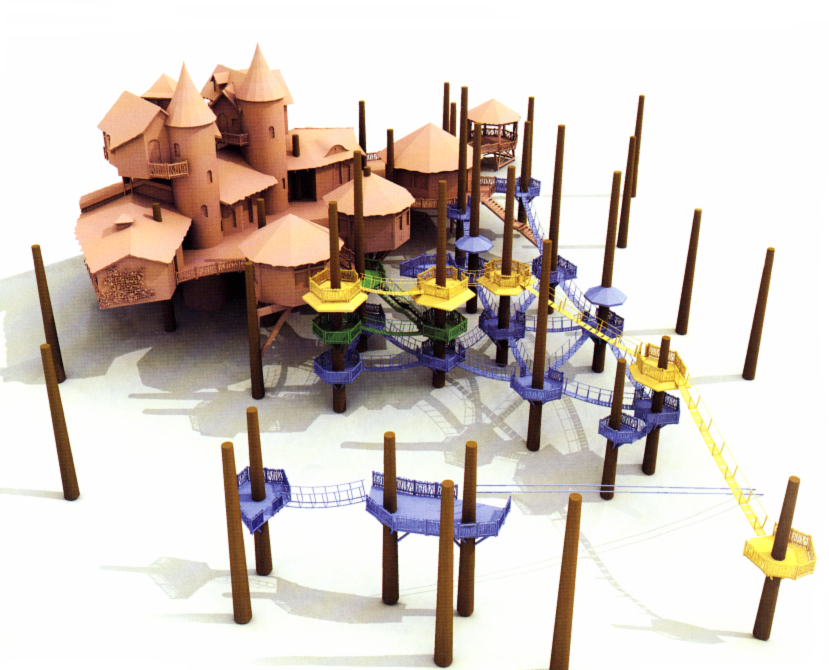
\includegraphics[width=400px]{images/titlepage_image.png}
\end{figure}
   
   
\end{titlepage} 
    %%%%%%%%%%%%%%%%%%%%%%%%%%%%%%%%%%%%%%%%%%%%%%%%%%%%%%%%%%%%%%%%%%%%%%%%%%%%%%%
    %   Abstracts                                                                 %
    %%%%%%%%%%%%%%%%%%%%%%%%%%%%%%%%%%%%%%%%%%%%%%%%%%%%%%%%%%%%%%%%%%%%%%%%%%%%%%%
    \setcounter{page}{1}
    \chapter*{Abstract\markboth{Abstract}{Abstract}}
    % Mark 'Abstract' both even and odd markers
    
    

\tableofcontents

\mainmatter
% Adjustments headers
\fancyhead[LO]{\leftmark}
\fancyhead[RE]{\emph{Chapter \thechapter}}

%chapter 1

\chapter{Introduction}
\label{sec:intro}

%This is a general introduction to what the thesis is all about -- it is not just a description of the contents of each section. Briefly summarize the question (you will be stating the %question in detail later), some of the reasons why it is a worthwhile question, and perhaps give an overview of your main results. This is a birds-eye view of the answers to the main %questions answered in the thesis.

Procedural modeling is an exciting research area with trumendous potential for virtual worlds. Virtual worlds range from games, to simulations and virtual communities. These worlds are often very large and with advances in technology and user demand they rapidily grow larger for each new application. The problem is that space in these vast virtual worlds needs to be filled with interesting content. Creating such high amounts of content by hand does provide nice job opportunities, but if we could generate the same content with a set of parameters and the push of a button the choice is rather obvious. However, time and money efficiency are not the only arguments for the development of procedural methods. By studying real world objects or sets of real world objects in order to dynamically synthesise them in virtual worlds we gain a deeper knowledge of the characteristics of these objects and relationships between different objects. 

A couple of succesful existing procedural modeling implementations are interesting to discuss. In games, procedural methods have been employed for the generation of worlds with restricted sets of environmental elements, such as dungeons and mazes. A good example is the game "Diablo 2". The game "Spore" was one of the first games that heavily utilized procedural modeling techniques for a considerable part of the content in the game. A very interesting project that is in development at the time of writing, is the game "Love" (figure \ref{fig:love}) developed by a single man. Procedural generation is used extensively for every part of this game.
      
\begin{figure}[htb]
\centering
\subfigure[World]{
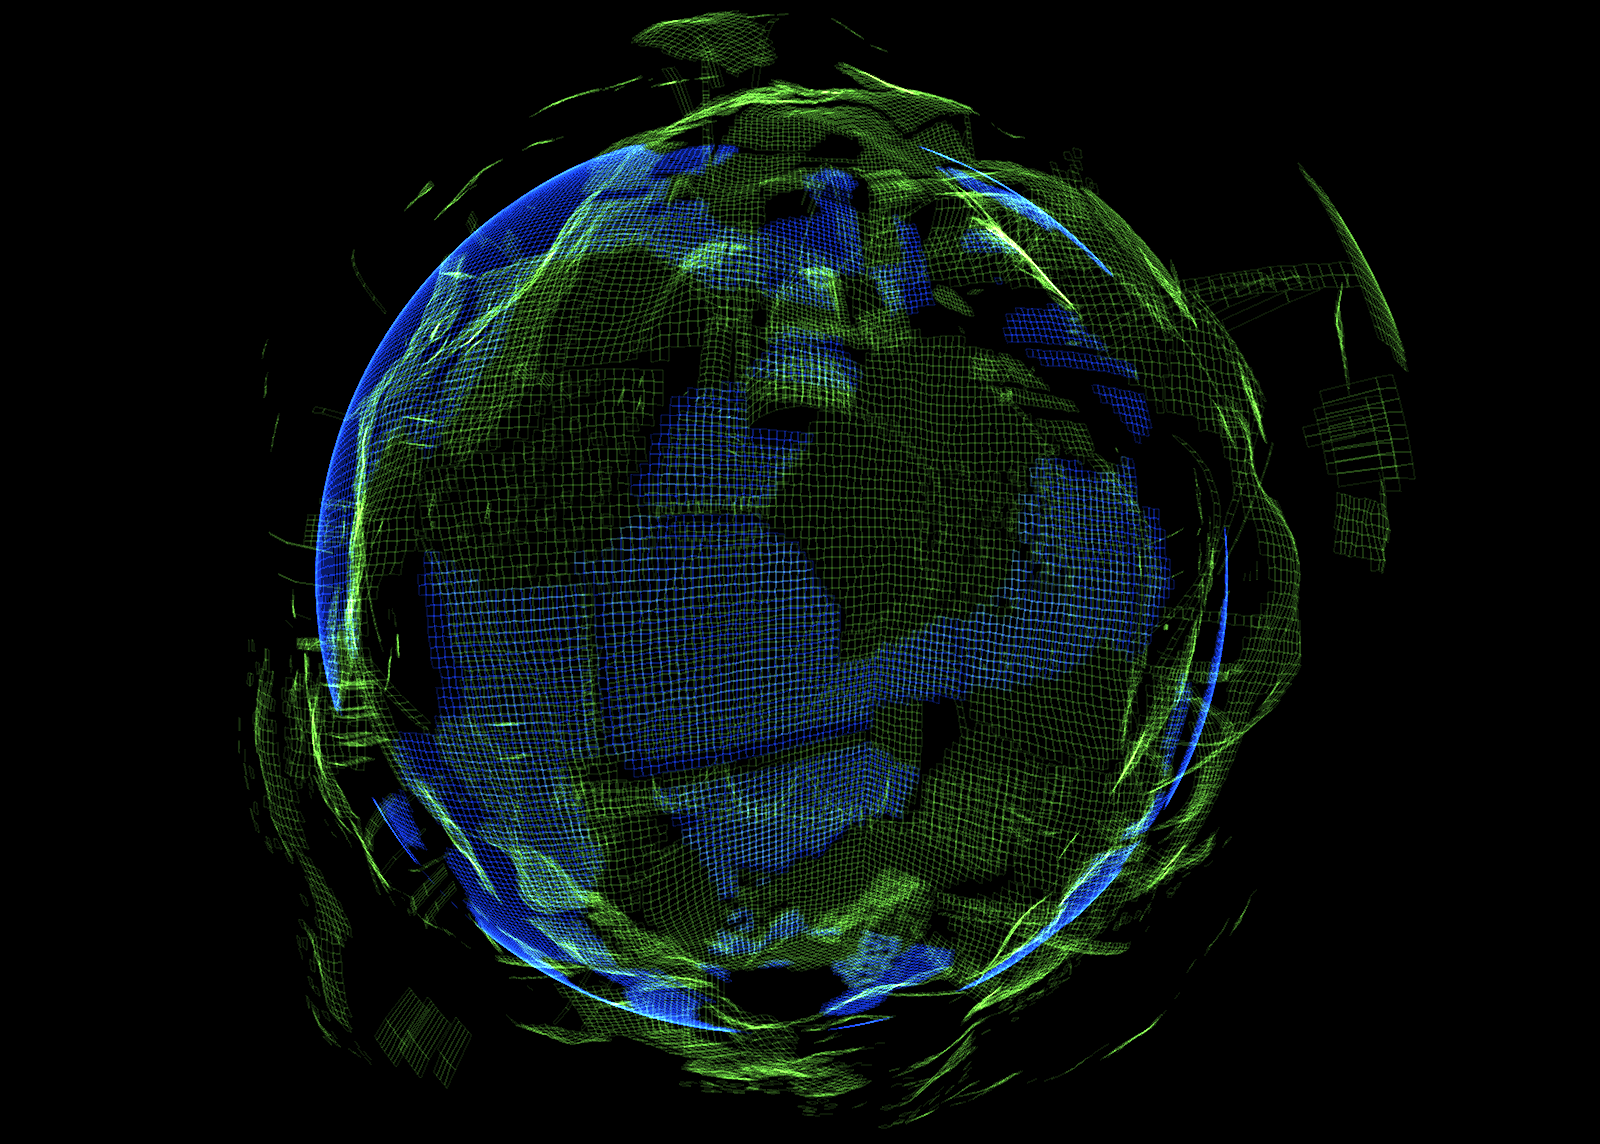
\includegraphics[width=100px]{images/love/world.png}
\label{fig:subfig1}
}

\subfigure[Ingame Environment]{
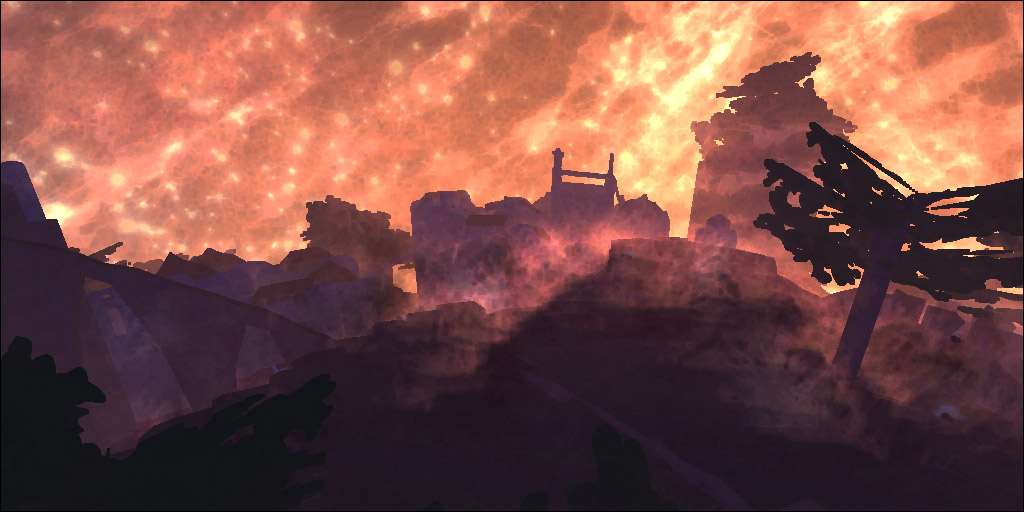
\includegraphics[width=100px]{images/love/love_city5.jpg}
\label{fig:subfig2}
}
\label{fig:love}
\caption[]{Screenshots of the game Love}
\end{figure}


This thesis adresses the problem of creating procedural architecture in the special case of restrictions and possibilities enforced by geometric properties of tree-like support-structures. A side goal for this research was to develop methods for intuitive interactive control for this specific procedural modeling method. 

%Regarding user control and procedural techniques it is important to strike a balance which allows for a fast %and intuitive building process, and meanwhile the user should have just the right amount of control to make the %scene to its liking.

%Rewriting systems, l-systems waarna shape grammars volgen
%The Shape grammar concept was originally coined by Stiny in his much cited \emph{"Shape and Shape Grammar"} \citep{Stiny80}.
%<hier de description van een shape>

Visual modeling of plant development is a field which started in 1962, when Ulam applied cellular automata to 
simulate the development of branching patterns \citep{PrzemyslawPlants}. A formalism for modeling plants was proposed by Lindenmayer 
in 1968, this formalism was called L-systems since. The following definition of an L-system is given by Przemyslaw \citep{PrzemyslawPlants}: 

\begin{quote}
An L-system is a parallel rewriting system operating on branching structures represented as bracketed strings of symbols with associated parameters, called modules. Matching pairs of square brackets enclose branches. Simulation begins with an  initial string called the axiom, and proceeds in a sequence of discrete deriviation steps. In each step, rewriting rules or productions replace all modules on the predeccesor string by succesor modules.   
\end{quote}   

Przemyslaw \citep{PrzemyslawPlants} has employed and extended the l-system formalism for realistic visualisation of entire plant ecosystems. Within a ecosystem organisms interact with each other and this interaction determines many properties for individual organisms; such as growth rate. Since the original L-system formalism does not account for communication between two processes, Przemyslaw proposed \emph{open l-systems} which incorporates \emph{communication modules}.    
  
L-systems also proved to be useful in the field of urban procedural generation \citep{Wonka03}. 
Muller showed that the L-system formalism could be succesfully used for the generation of road networks and in lesser extent building generation. 

%hier wat over building, generation, city generatoin, texture generation.
%shape grammars

Techniques for tree generation in this thesis are based on L-systems, however these techniques are simplified to a certain degree since the modeling of plants is not the maintopic of this thesis. We have used the l-system formalism to generate simple branching tree structures. We did not strive to generate visually realistic models of trees since this has already been achieved by many people before me with impressive results. Instead our simplified method generates the main structure of a tree which is then used as input in our method to generate configurations of architectural elements. 

%<hier resultaat van treehouse generatie module>

It is the case that traditional general purpose modeling software is very time consuming for the creation of complex scenes as a result of the lowlevel tools they feature. Special purpose modeling tools such as cityEngine \citep{Muller06} (in the case of urban modeling) and speedTree (in the case of modeling plants and trees) provide procedural methods to generate objects within a certain class with very high time effiency. However the human touch still remains a very important part of the modeling procedure. Eastatics are very hard to turn into a set of formal rules on which an algorithm can operate.

The special purpose modeling tool for the generation of organic geometry and treehouse architecture that was developed for this thesis provides the user with intuitive interaction tools to allow easy manipulation.        


%\old{   
%The research which preceded this document strived to construct an intuitive organic modelling method for the creation of 2D maps. The central focus of this research has been on methods %for construction of dynamic structures using real-time growth models. To enable a large degree of control over these dynamic structures the is a need for skeletons. A large part of this %thesis is about constructing skeleton representations for dynamic structures. There obviously is a realtime demand in order to enable realtime interactivity, which means building such %skeletons should above all be an efficient process.    
%}

\section{Overview}
\label{subsec:overview}

This thesis is structured as follows. In the next section I will discuss related work. In the related work section I will bring my thesis into context with regard to procedural modeling of trees, architecture and generation of levelmaps. A precise statement of the problem and why it's an interesting problem to solve will follow in section \ref{sec:problem}. 

In section \ref{sec:concept} I will present the conceptual system model. The method for the generation of the forest layout and the generation of the tree geometry is presented in section \ref{sec:pfg}.  
 
With the forest geometry in place we are ready to review the planning method which is responsible for the construction of a connected graph representing a tree community. I will conclude the method description with a look at the final stage of the pipeline, translating the symbols from the nodes and edges of the graph to the geometrical architectural elements. Section \ref{sec:UIT} discusses user interactivity and usability of the proposed system. The last two sections present results and conclusions respectively.     

%chapter 2

\chapter{State of the Art in Procedural Modeling}
\label{sec:relatedwork}

%plants 

\section{Plants and Trees}
Algorithmic Beauty of Plants by Lindenmayer and Przemyslaw \citep{PrzemyslawAlgoBeauty} is the first complete work discussing the generation of plant geometry using procedural methods such as L-systems and fractals. To model and visualise realistic ecosystems, Przemyslaw extended the l-systems concept to a system which allowed communication between systems (open l-systems \citep{PrzemyslawPlants} \citep{Deussen98}). Visual editing of procedural plants models is discussed in \citet{interactivebonsai}. 

%road networks
\section{Road Networks}
The foundation for procedural city and building modeling was provided by Parish and Muller \citet{Parish01} in their paper \emph{"Procedural Modeling of Cities"}. The main contribution of this paper is the use of extended L-systems for the generation of city roadmaps. They also propose a method for the texturing of facades. An intuitive editing approach for road networks with the use of tensor fields and bush techniques is presented by Chen et al. \citet{Chen08}. 

%building architecture
\section{Architecture}
An attempt was made to use L-systems for the creation of buildings \citet{Parish01}, however this did not prove to be effective. L-systems are designed to handle growth-like processes, it has been acknowledged that the construction process of a building is not a growth like process. Instead, building construction is better expressed by series of partitioning steps. These partitioning steps can be described by another kind of rewriting grammar called \emph{set grammar}. In \citet{Wonka03} Wonka presents a method for the automatic creation of building using such grammar systems. In this work Wonka introduces the idea of a specialized type of set grammar called \emph{split grammar} which operates on shapes. In \citet{Muller06} the split rules from the split grammar concept are defined in a grammar system called \emph{CGA Shape}, which was the first procedural system for the creation of detailed buildings with consistent mass 
models. The process of creating a ruleset in CGA shape for a specific type of building is not straightforward and requires a trained expert. Lipp et al. \citet{Lipp08} introduce a visual method for the editing of the CGA Shape grammar for procedural architecture to simplify the rule building process.

\section{Procedural Game Worlds}
%content here%


%chapter 3
\chapter{Problem Statement}
\label{sec:problem}


%1. a concise statement of the question that your thesis tackles
The purpose of this thesis is to tackle a specific instance of the problem of planning connected architectural geometric elements into an environment with existing geometry which is to be used as the supporting structure for the architectural elements. We handle the specific case in which the pre-existing geometry is a virtual forest, using the trunks and branches of the trees as supporting structures for architectural elements such as platforms, bridges, stairs and buildings. We propose several heuristics for the generation of a connected 'tree house community' and using these heuristics we propose a planning algorithm. The architectural elements need a large degree of adjustibility to be able to incorporate them into the irregular environment posed by the tree geometry, therefore we present procedural methods for the generation of these elements. Another goal for this thesis was the design of intuitive procedural modeling user tools.      

This work has been inspired by advancements in the fields of procedural plant generation and procedural generation of urban structures like buildings, roads and entire cities. These two fields have been explored to some extent now. Although the generation of urban structures is a relatively new research area compared to procedural plant generation. Never before have these fields been combined for our idea: the generation of architectural geometry controlled and supported by tree-like geometry. With our research we attempt to 
generate interesting meaningful \emph{'tree-house community'} scenes.

%3. discussion of why it is worthwhile to answer this question.
I believe this is an interesting problem to be solved for the following reason. Previous solutions for procedural virtual worlds focussed on realistic synthesis of the real world around us. In games, virtual worlds are designed with high user-entertainment value as top priority. This also means that the configuration of geometry in virtual game worlds must enable the user to enjoy the playing experience. Determining the leveldesign principles that make a virtual world enjoyable is hard on its own. Transforming these principles into formal rulesets is even harder. To make the problem even more complex, the principles for good leveldesign highly depend on the game play rules the virtual world dictates. We present two scenarios that incorporate a set of gameplay rules. From these scenarios and known pricipals of good leveldesign we create heuristics. Using these heuristics we construct a planning algorithm that takes forest geometry, a set of architectural elements and parameters we extracted from the scenarios as input and outputs a geometric configuration of the architectural elements.     

An important inspiration for our research is work done on the procedural generation of dungeons. 

%Although popular techniques for creating plants (prezmyslaw) and buildings (Muller) show similarities, there are some important %differences.     
%chapter 4 

\chapter{Concept}
\label{sec:concept}

%dit is in feite het idee,bladiebladiebla

This section discusses the concept for the proposed procedural modeling method with main focus to the planning algorithm for architectural objects. 




%Figure \ref{fig:conceptualmodel} shows a diagram of the proposed system.
%
%\begin{figure}[htbp]
%	\centering
%	\caption{diagram of the conceptual model}
%	\label{fig:conceptualmodel}
%\end{figure}







%chapter 5


\chapter{Schematic Outlay Generation for Elements}
\label{sec:schematicoutlay}

%\begin{quotation}
%�Chaos in the world brings uneasiness, but it also allows the opportunity for creativity and growth.�
%\caption{Tom Barrett}
%\end{quatation}





%l-system uitleg hier 

I am interested in the structure of trees and the possibilities and restrictions it poses for placement of 
architectural shapes. For the purpose of this thesis the generated trees do not have to be visually convincing, however the basic shape should still be identified as a tree. The geometric properties of a tree model that are to interest of us are those that have effect on the possibilities with respect to the incorporation of architectural man-made structures. The tree geometry functions as the support structure for the building blocks I define in detail in section \ref{sec:treehousearch}. 

In this section we will discuss a method that generates a graph representing the structure of elements in a forest environment.  


\section{Scattering Techniques for Tree Positions}
\label{sec:scattering}

\section{Ecosystem Modeling}


\section{Multilayer TreeNode Generation}

%Previous plant ecosystem generation techniques were mainly focused at generating visually realistic con 

%todo: alter
For our method we have to be able to strategically place geometric architectural elements within tree structures. Finding the positions at which these architectural elements can be placed could be performed as a postprocess type process by analyzing the generated geometry, however we have the oppertunity to incorporate positional semantic information to the trees during the generation phase which simplifies the problem. 

L-system tree generation methods are mainly focused at producing convincing visual representations of trees \citep{Prezmyslaw}. However, we do believe that these methods can be extended quite easily to enable the addition of structural semantics. This thesis does not pursue the introduction of such an extension. For our problem we mainly have to deal with structure of a forest which we will abstract to a set of nodes, representing trees, for the moment. Finding useful connections between nodes and incorporation of structual elements within these tree nodes is what we are interested in.    

We propose a multilayer graphbased approach for the generation of a schematic outlay for elements in a forest structure. The nodes in this structure function as empty slots which define semantics that determine the type of elements this node can contain. See figure \ref{fig:treenodes} for an example element graph for a single tree.    

The element properties of a node are used to query the architectural element database. Listing \ref{list:properties} shows an example of element properties for a node. 

\lstset{language=Java, caption=Example of node element properties, label=list:properties, basicstyle=\footnotesize,
frame=shadowbox, rulesepcolor=\color{black}}

\newpage

\begin{lstlisting}

Element_node_14
{
	single_node_platform
	{
		available = true; 
		max_diameter = 30.0;
	}
	
	bridge
	{
		available = false; 
		type = suspension;
	}
	
	multi_node_platform
	{
		available = true; 
		other_nodes = array{34, 23, 78};
		type = undefined;
	
	 if (used)
	 		bridge.available = true;
	 else
	 		bridge.available = false; 		
	
	} 
	
	building
	{
		available = false;
	}
	
	stairs
	{	//staircase connection to parent node
		available = true; 
		type= revolving; 
	}
}

\end{lstlisting}

I will cover node element properties and quering of the element database in the next chapter in more detail.   

%The global forest schematic consists of a set of tree element schematics which have been scattered on a plane using the scattering technique discussed in the %previous section. The schematic of the forest includes all possible connections (bridges) between element graphs. Nodes in an element graph of a tree are contained %in a layer that contains the nodes positioned at the same height in all trees of the forest. The number of layers is determined by the element graph with highest %node level.  

%The height ($z$ coordinate) of a node is determined by the height property of the containing layer, while the position of a node in the plane defined by the layer %represents the $x,y$ coordinate of the branch.  

Our schematic outlay generation method uses the following parameters: 

\begin{enumerate}
\item Area  $A$  
\item Density $D (0.0 < D < 1.0)$  
\item Layers $L (L > 0)$ 
\item Tree parameters defining min bounds $T_{min}$
\item Tree parameters defining max bounds $T_{max}$
\item LocalTreeDeviation (controls deviation of tree properties within an area of size ClusterArea)
\item ClusterArea
%\item GlobalTreeDeviation
\end{enumerate}

%quick overview
With these parameters in place I can start discussing the algorithm. The rootnodes of our tree element graphs are contained by the base layer. The algorithm start by assigning 2d coordinates to the root nodes of each element graph using the scattering algorithm.

The scattering algorithm requires the $Area$, $Density$ parameters and the bounding $Tree parameters$ which determine the actionradius for
the generated trees. For each root node the algorithm sets a semi-random parameterset $P_t$ ($T_{min} < P_t < T_{max}$). The second step of the algorithm creates the upper $L-1$ layers. 

A layer is in fact a container for element nodes of all trees that allow connections through bridging. Nodes within a single layer roughly have the same height to the baselayer. Whether two nodes within a layer can be connected with a direct bridge depends on the element element properties of these nodes, the distance between them, and obstructions caused by other nodes.   

With the layers in place we iterate through the root node list in the base layer. For each root node a corresponding element graph is build. The method that builds an element graph depends on the global parameters of the forest but also on the structure of local neighbours. The method performs local statistical analysis on local element graphs within an area of size $ClusterArea$, and the result, combined with the $LocalTreeDeviation$ parameter, is used to generate a deviating tree element graph. Again note that the nodes in the element graph provide information about allowed architectural elements at this node, and the edges of an element graph represent connections by means of stairs or bridges. The element graph is in fact a subgraph of the final tree-structure graph that I will discuss in section \ref{sec:ElementToTree}.    

Growing an element graph for a tree means iterating through the layers. For each layer, $n$ ($0>= n >MaxNodes$) nodes with element properties are generated (a pointer to each node is stored in the local tree element graph and the corresponding layer). Note that when the element graph has no nodes at a specific layer this does not mean that the graph has stopped growing. Instead it means that the final tree structure prohibits elements to be placed at this position. When a new node is added to a layer the method tries to connect it to local nodes, provided that the node allows bridge connections. Figure \ref{fig:layers} shows a configuration of element graphs.

\begin{figure}[h]
	\centering
		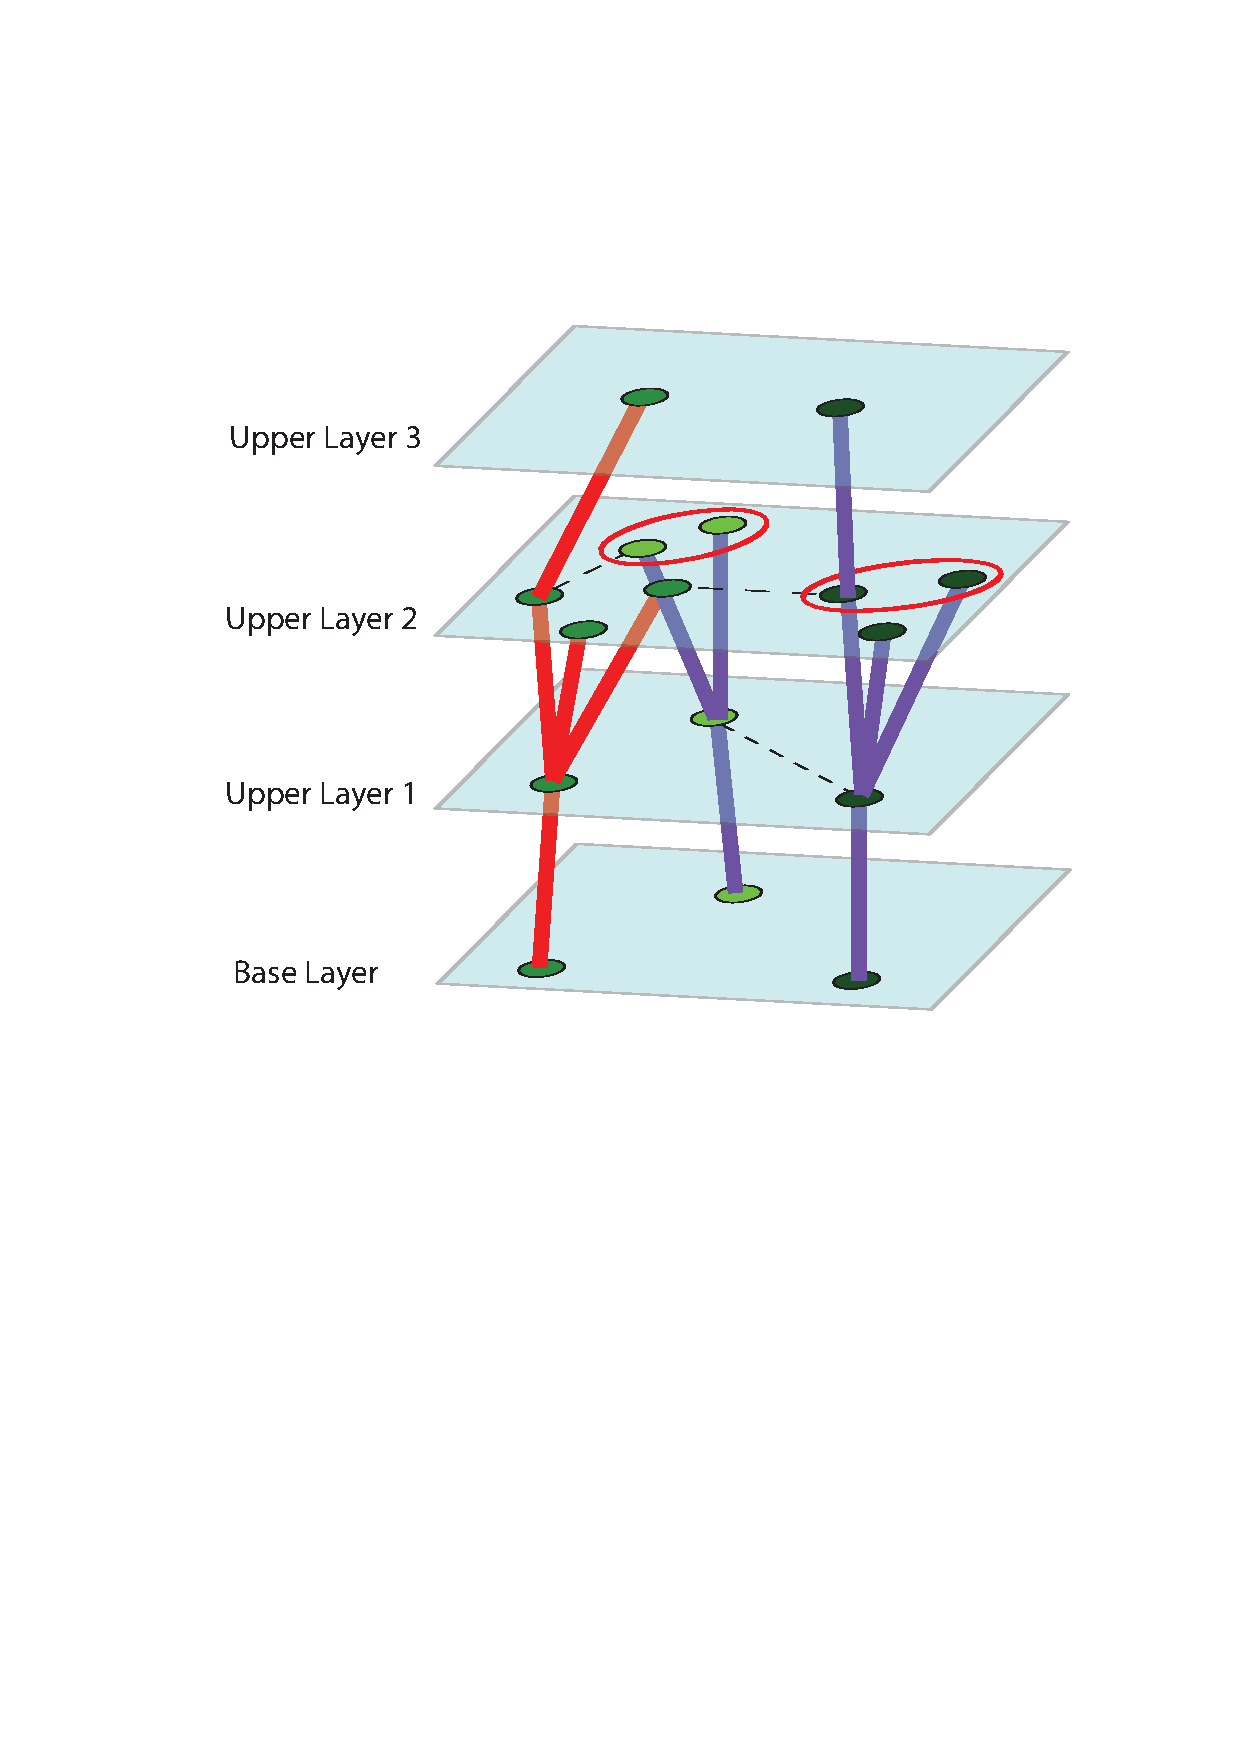
\includegraphics[width=220px]{images/element_graph_layers.pdf}
	\caption{example of multilayer element graphs for a small tree set}
	\label{fig:layers_and_graphs}
\end{figure}

When all element nodes have been constructed and placed into corresponding tree element graphs and layer element graphs the method checks wether all nodes are reachable from any other nodes. Single nodes or sets of connected nodes that are not reachable from the the main node graph will be deleted. We now have the schematic structure of a forest which we need as input for the architecture planning method discussed in the next section.          

% For every node $n_i$ contained by the base layer the method performs the folowing steps:  

%\begin{enumerate}
%\item Step1: 
%\item Step2:
%\item Step3:
%\item Step4:
%\end{enumerate}


%%%%%


%wat moet er nog in:


%- geven we de boom met een aparte node weer?	
%- wat nou als een platform support wordt door meerdere bomen -> meerdere nodes 
%		mogelijke oplossing: als een set van nodes een platform ondersteund, deze nodes als 1 node 
%   behandelen, dus zijn er twee graphs nodig. 1 voor alle nodes, 2e voor graph waarin bepaalde platformnodes samen worden gevoegd tot 1 node.   
 
%- hoe wordt een boom graph opgebouwd?
%- per upper layer is er voor elke branch een bounding area waar het in terecht kan komen
%- vaststellen van mogelijke connecties (bruggen) 
%- proces volgorde: eerst bepalen welke elementen we willen kunnen plaatsen in de boom
%- hoe beschrijft de semantiek welke elementen kunnen worden geplaatst? 

\newpage
\subsection{Simple Tree Structure}

Procedurally generating trees by means of l-systems has had a great amount of succes since the original proposal by Lindenmayer. The L-system formalism is widely applied in  academic work and is also succesfully used within commercial applications. This thesis does not focus on the l-system formalism in particular, since it is already a well established theory \citet{PrzemyslawAlgoBeauty}. I describe L-system in short in the following section as it is the most used fomalism for the contruction of trees.  


\subsection{Creating Tree Geometry}



 
%%%%%%%%%%%%%%%%%%%




%%%%%%%%%%%%%%%%%%%






%After construction of the multilayer graph representation of the forest, we feed it to the architecture planning algorithm that is discussed in section %\ref{sec:architecture}. 



%calculation of interval here     

%The first step of the method involves creation of $n$ ($0 <n < MAX_LAYERS$) layers.          
%The trunk node of every tree is placed inside the base layer.
%We will eventually translate the node based configuration of a forest to a visual representation   
%Therefore we propose an alternative method for the generation of forests as previous forest generation %methods do not incorporate semantic information  
%We propose an alternative method for the generation of forest geometry which supports    

%chapter 6

\chapter{Planning Game World Structure}
\label{sec:treehousearch}
 
  
\section{Background}
%About patterns in city architecture and buildings
%patterns in biology 

%
%patterns in game worlds: dungeons
%


In the next section I discuss literature on characteristics of succesfull leveldesign in games.  

\section{Considerations on Leveldesign in Games}

% 
%
%
%
%

\chapter{Formalization of Game World Structure Patterns}
\label{sec:scenarios}


\section{Scenarios} 
In the next three sections we define game world scenarios that could occupate the generated forest structure. Each of the scenarios we propose here is based on a popular videogame genre: 

\begin{enumerate}
\item Puzzle / Adventure Dungeon
\item 3rd Person Strategy 
\item 1st Person Shooter
\end{enumerate} 


\section{Scenario 1: Puzzle / Adventure Dungeon}
Leveldesign Patterns in Puzzle and Adventure Dungeons:

\begin{itemize}
\item circular paths, loops. Example: The player arrives at a door and it is locked, you must take a different route and along the way you find a key. Now the player heads back to the door through which he can now proceed.  
\item start at bottom, move to top. It is almost always the case that dungeons have multiple floors. The player starts at the bottom floor and progressing through the dungeon means moving up to a higher floor.      
\item re-using different paths by opening new door and locking old ones.    
\item no path deviation. Rules for movement are very strict in these type of games.

\end{itemize}

%\section{Planning Algorithm for Scenario 1}


\section{Scenario 2: 3rd Person Strategy}


% hoe begint het algoritme?
% wat zijn de parameters? 
% 
%
%
%


%\section{Planning Algorithm for Scenario 2}

% hoe begint het algoritme?
% 
%
%
%
%


%\section{Scenario 3: 1st Person Shooter Multiplayer Arenas}

\begin{figure}[ht]
\centering
\subfigure[]{
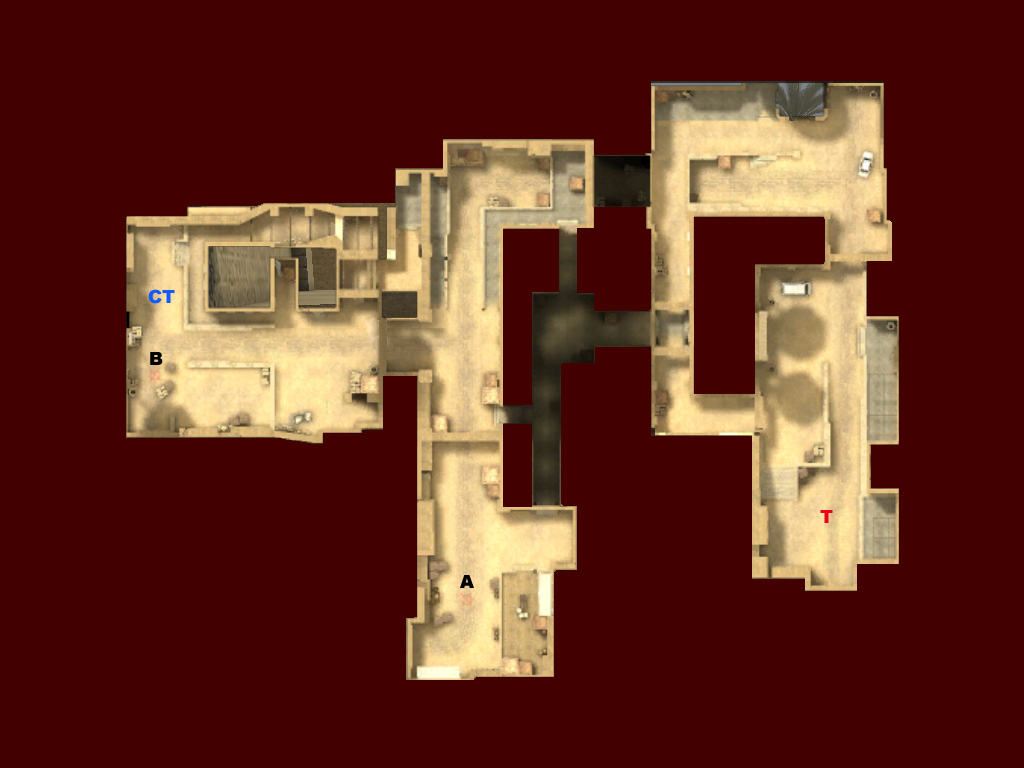
\includegraphics[width=300px]{images/game_maps/de_dust_overhead_2.jpg}
\label{fig:subfig1}
}
\subfigure[]{
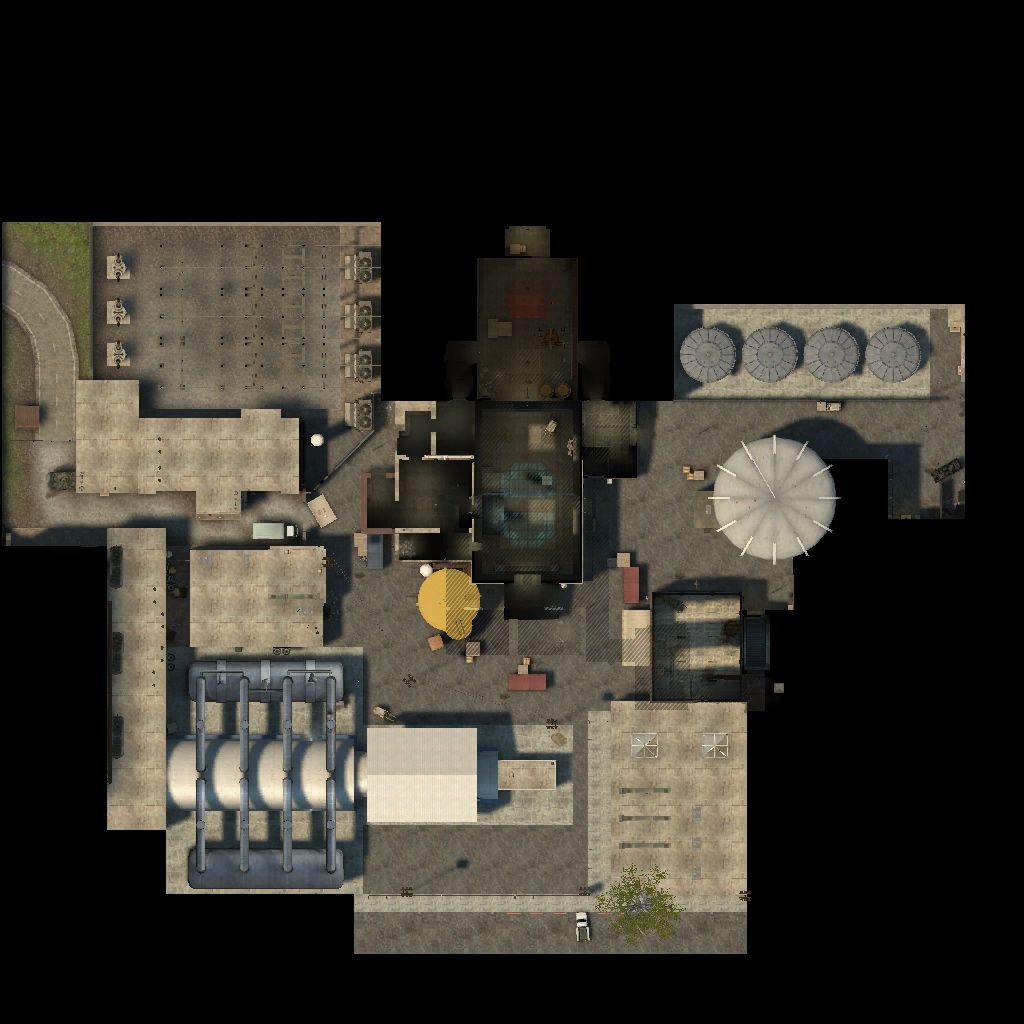
\includegraphics[width=300px]{images/game_maps/de_nuke.jpg}
\label{fig:subfig2}
}
\label{fig:fpsmaps}
\caption[Overview of classic FPS maps(from the game Counterstrike:Source). The "Multiple paths" pattern is clearly visible.]{}
\end{figure}

\subsection{symmetry}

\subsection{Multiple paths}

\subsection{Local fights}

\subsection{Collision points}

\subsection{Reference points}
	
\subsection{Defense areas}

\subsection{Risk Incentive}

%\section{Planning Algorithm for Scenario 3}

% hoe begint het algoritme?
% 
%
%
%
%

%From the scenarios I discussed in the previous section we can extract a set of parameters and goals for our algorithms.
\chapter{Planning Algorithms}

\section{Considerations}

\section{Planning Methods}

%
%
%
%
\label{sec:PlanningAlgorithm} 
  
 Using the scenarios and architectural elements we have defined in the previous section we will formulate our planning algorithm now.
 I will first introduce the planning algorithm informally followed by a more formal approach.
      
  
%\begin{algorithm}
%\caption{The planning algorithm}
%\begin{algorithmic}
%\IF {$i\geq maxval$} 
%        \STATE $i\gets 0$
%\ELSE
%        \IF {$i+k\leq maxval$}
%                \STATE $i\gets i+k$
%        \ENDIF
%\ENDIF 
%\end{algorithmic}
%\end{algorithm}


\chapter{Geometry Generation}

\section{Procedural Generation of Architecture Geometry} 
\label{sec:archelements}
 
%nog iets moois hiervoor 
In this section we present the geometrical elements we use for the construction of our treebased architecture. We will first introduce the elements in a broad sense, followed by descriptions of methods to construct the geometry of some of these elements procedurally. 
 
\subsection{The Element Vocabulary}
We established a set of architectural elements we believe are the most basic tree-based architectural structures: 

\begin{enumerate}
\item Platforms
\item Buildings
\item Bridges 
\item Stairs
\item Miscellaneous Elements 
\end{enumerate} 

\begin{figure}[ht]
\centering
\subfigure[Platform]{
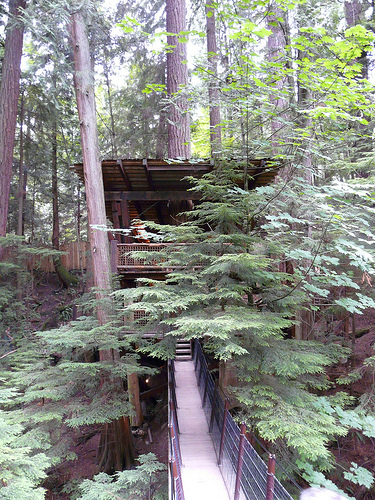
\includegraphics[width=50px]{images/platform.jpg}
\label{fig:subfig1}
}
\subfigure[House]{
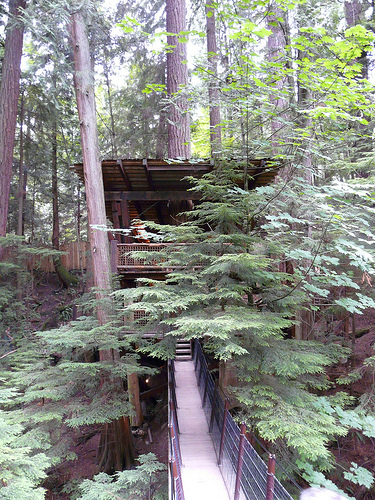
\includegraphics[width=50px]{images/house.jpg}
\label{fig:subfig2}
}
\subfigure[Bridge]{
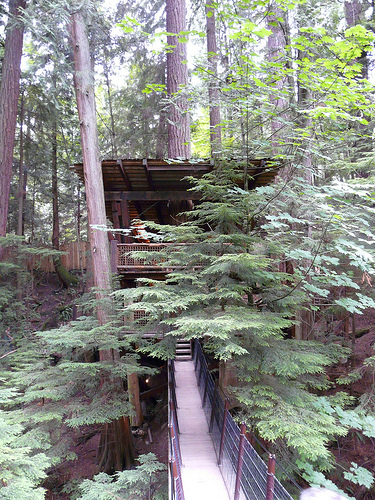
\includegraphics[width=50px]{images/bridge.jpg}
\label{fig:subfig3}
}
\subfigure[Stairs]{
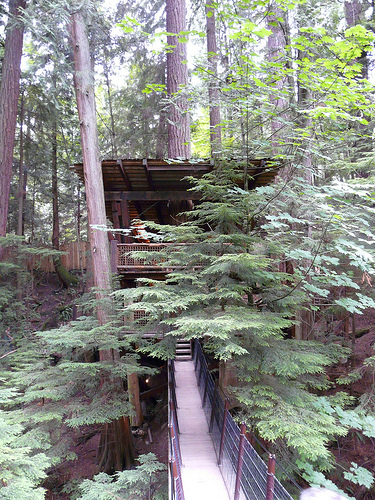
\includegraphics[width=50px]{images/stairs.jpg}
\label{fig:subfig3}
}
\label{fig:archElements}
\caption[Architectural Elements Vocabulary]{Caption of subfigures \subref{fig:subfig1}, \subref{fig:subfig2} and \subref{fig:subfig3}}
\end{figure}


 
\subsection{Platforms}
\label{sec:platform}
 


\subsection{Housing}
\label{sec:building}




\subsection{Bridges}
\label{sec:bridges}





\begin{figure}[ht]
\centering
\includegraphics[width=200px]{images/suspension-bridge.jpg}
\label{fig:bridgeExample}
\caption{A typical suspension bridge}
\end{figure}
The curved surface of a suspension bridge can easily be described with a spline.   

\subsection{Stairs}
\label{sec:stairs}
  
We define two types of stairs. The first is the simple vertical linear stairs-type. The second is the revolving staircase, which revolves around a tree trunk like a corkskrew. 


%\subsection{Connecting Elements} 
%
%We construct an architectural structure by combining the elements we have in our element vocabulary.
%In order to construct logical combinations we need to define for each elements how it can be joined with other elements
%in our vocabulary.

  
%chapter 7 (optional)

\chapter{User Interaction Tools}
\label{sec:UIT}

\section{Growing Surfaces}
\label{sec:GrowingSurfaces}

%Per type spatial growth model bespreken wat de context is binnen outdoor areas en dus met 
%welke andere spatial growth modellen het communiceert en welke effecten het spatial growth model heeft 
%op de andere en vica versa. Ook bespreken op wat voor manier een vector field (en andere tools 
%die invloed hebben op de ruimtelijke indeling)  effect heeft op de uitdijing van dit type model.   


%A definition of land: "The part of Earth which is not covered by oceans or other bodies of water".(bron: %http://en.wiktionary.org/wiki/land ...jaja ik vind nog wel een betere bron)
%In reality land obviously does not grow, so first we must ask ourselves whether growing land in our virtual %world can be made useful and intuitive to use. There are no real rules for the bounding shape of a piece of %land, the bounds can be configured in any way. However due to this fact almost any random configuration of the %shape of land looks realistic. The question is, as with other growth models with a minimum amount of rules, %whether generating land by means of a growth model, thereby having less control over the result compared to %conventional methods, is something which we want. 

%When you want maximum control over the resulting geometry of a piece of land, using a growth model is not a %very attractive method.However there are some situations in which this method is quite helpful.

%\inhoud
%{wanneer is het groeien van land handig: 
%\begin{itemize}
%\item Obviously: In situaties waarin de gebruiker niet veel waarde hecht aan de precieze vorm van de resulterence geometrie.  
%\end{itemize}
%}

%Land provides the underlying surface of many of the growth models discussed in this paper. 

%\inhoud
%{dus het bestaan van land op de seedpositie van een afhankelijk groeiproces is een eis. Wellicht moet het genereren van een map bestaan uit verschillende fases:
%\begin{itemize}
%\item fase 1: generatie van land en water. 
%\item fase 2: plaatsen en activeren van groei processen die afhankelijk zijn van land.  
%\end{itemize}
%}

%The field of biological modeling provides some interesting modeling techniques for the process of cell division. 
%Cell division is interesting with respect to the concept of growing land because it is an expanding process with some nice properties. \voegtoe{benoem properties of revise deze zin.} 


\section{Vector and tensor fields}
\label{subsec:vectorfields}

%\inhoud{
%\begin{itemize}
%\item vector fields: dit moet je wellicht helemaal aan het begin doen omdat alle spatial growth models
%gemanipuleerd worden door deze vector fields.
%\item obstruction with solid objects
%\item smudge-like tool
%\end{itemize}
%}

 
%chapter 8 Results 

\chapter{Results}
\label{sec:results}


\section{Empirical study of the results}

%chapter 9 conclusion
\chapter{Conclusion}
\label{sec:conclusion}



\appendix
%\noappendicestocpagenum
%\addappheadtotoc

% Adjustments headers
\pagestyle{fancy}
\fancyhead[LO]{\leftmark}
\fancyhead[RE]{\emph{Appendix \thechapter}}
\renewcommand{\headrulewidth}{0.5pt}

%\chapter*{Appendix A: Implementation}
%\label{sec:implementation}

%\chapter*{Appendix B: Application Class Structure}

\newpage 
\pagestyle{plain}
\addcontentsline{toc}{chapter}{Bibliography}
\bibliographystyle{abbrv}	% (uses file "plain.bst")
\bibliography{thesisrefs}	% expects file "myrefs.bib"

\end{document}

